\documentclass{beamer}
\usepackage[english, russian]{babel}
\usepackage[T2A]{fontenc}
\usepackage[utf8]{inputenc}
\usepackage{indentfirst}
\usepackage{amsmath, amsfonts, amssymb, amsthm, mathtools}
\usepackage[export]{adjustbox}
\usepackage{graphicx} 
\graphicspath{ {./images/} }

\usepackage{subcaption}
\usepackage{verbatim}

\usepackage{minted}{\setlength{\parskip}{0pt}}

\usepackage{hyperref}

\hypersetup{
    colorlinks=true,
    linkcolor=blue,
    filecolor=magenta,      
    urlcolor=black,
    pdftitle={Overleaf Example},
    pdfpagemode=FullScreen,
    }


\title{Лабораторная работа № 12. \\Синхронизация времени}
\author{Данила Стариков \\ НПИбд-02-22}
\institute{Российский университет дружбы народов имени Патриса Лумумбы}
\date{2024}

\begin{document}

\frame{\titlepage}

\begin{frame}
  \frametitle{Цель работы}
  \begin{itemize}
  \item Получение навыков по управлению системным временем и настройке синхронизации времени.
  \end{itemize}
\end{frame}

\begin{frame}
  \frametitle{Настройка параметров времени}
  \centering
  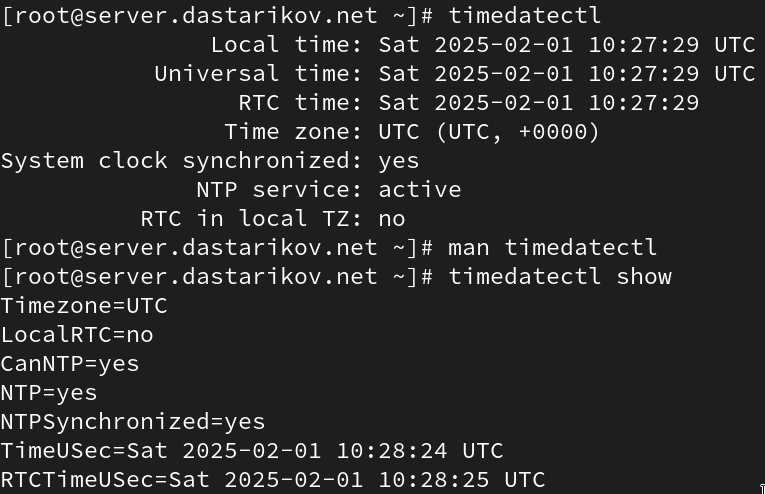
\includegraphics[width=\textwidth]{../images/image01.png}
  \captionof{figure}{Информация о дате и времени на сервере (timedatectl).}
\end{frame}

\begin{frame}
  \frametitle{Настройка параметров времени}
  \centering
  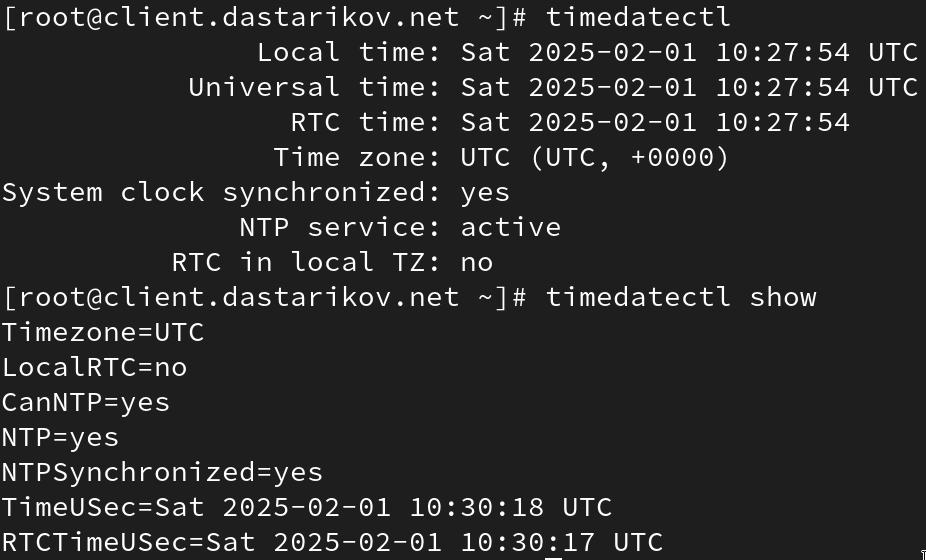
\includegraphics[width=\textwidth]{../images/image02.png}
  \captionof{figure}{Информация о дате и времени на клиенте (timedatectl).}
\end{frame}

\begin{frame}
  \frametitle{Настройка параметров времени}
  \centering
  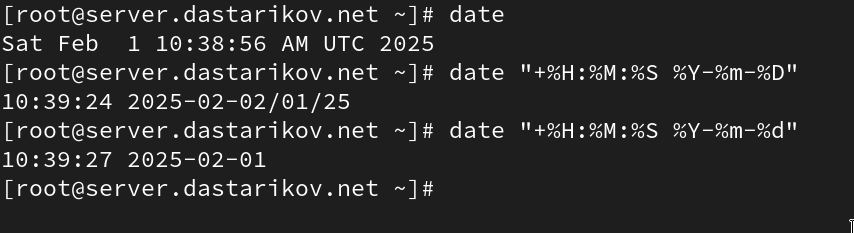
\includegraphics[width=\textwidth]{../images/image04.png}
  \captionof{figure}{Вывод команды \texttt{date} с разными ключами на сервере.}
\end{frame}

\begin{frame}
  \frametitle{Настройка параметров времени}
  \centering
  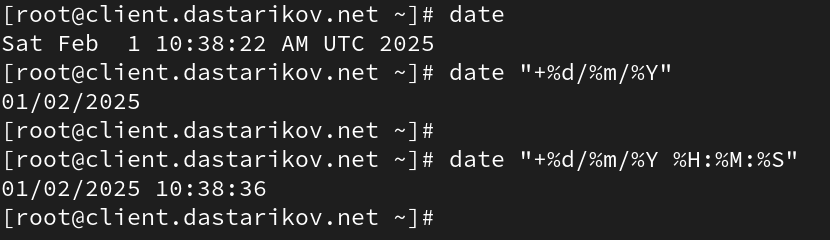
\includegraphics[width=\textwidth]{../images/image03.png}
  \captionof{figure}{Вывод команды \texttt{date} с разными ключами на клиенте.}
\end{frame}

\begin{frame}
  \frametitle{Настройка параметров времени}
  \centering
  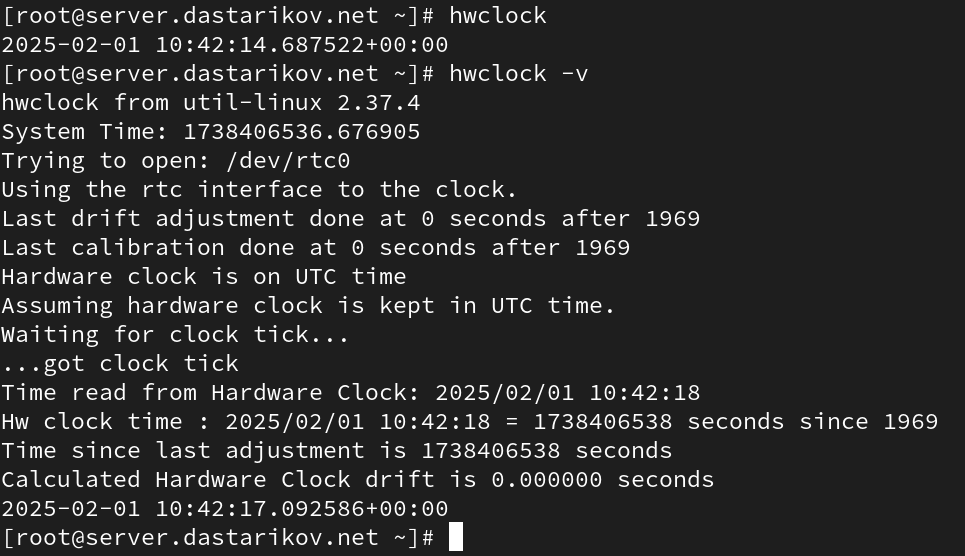
\includegraphics[width=\textwidth]{../images/image07.png}
  \captionof{figure}{Вывод команды \texttt{hwclock} с разными ключами на сервере.}
\end{frame}

\begin{frame}
  \frametitle{Настройка параметров времени}
    \centering
    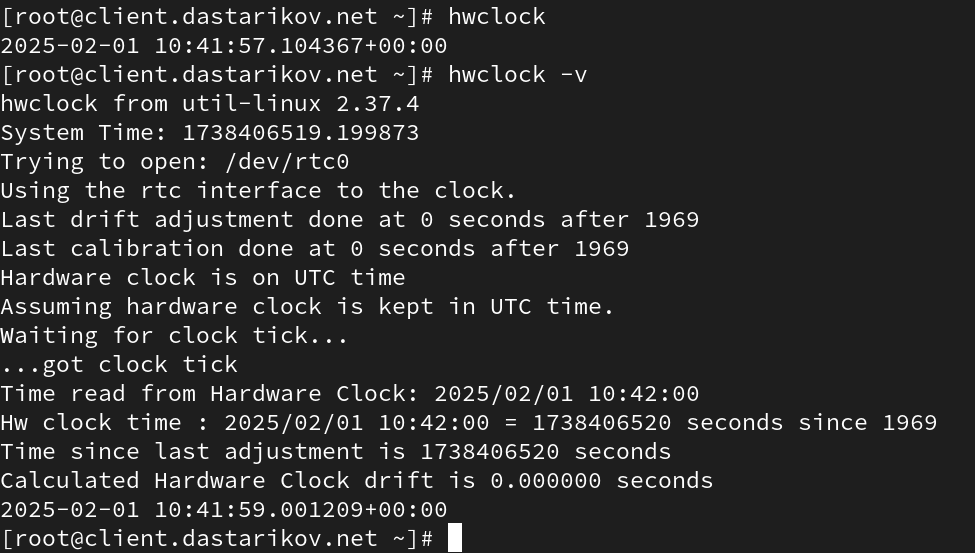
\includegraphics[width=\textwidth]{../images/image06.png}
    \captionof{figure}{Вывод команды \texttt{hwclock} с разными ключами на клиенте.}
\end{frame}

\begin{frame}[fragile]
\frametitle{Управление синхронизацией времени}
  \begin{minted}{bash}
    dnf -y install chrony
  \end{minted}
    \centering
    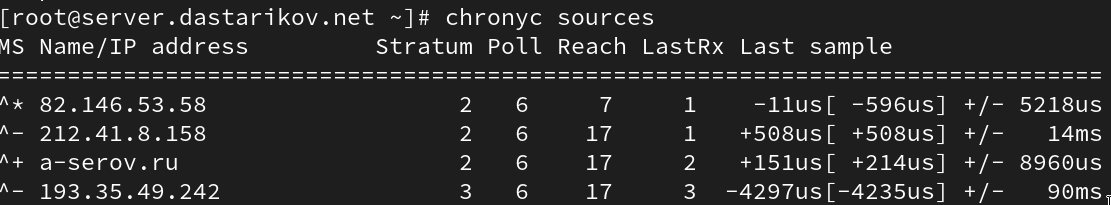
\includegraphics[width=\textwidth]{../images/image08.png}
    \captionof{figure}{Проверка источников времени на сервере.}
\end{frame}

\begin{frame}
\frametitle{Управление синхронизацией времени}
    \centering
    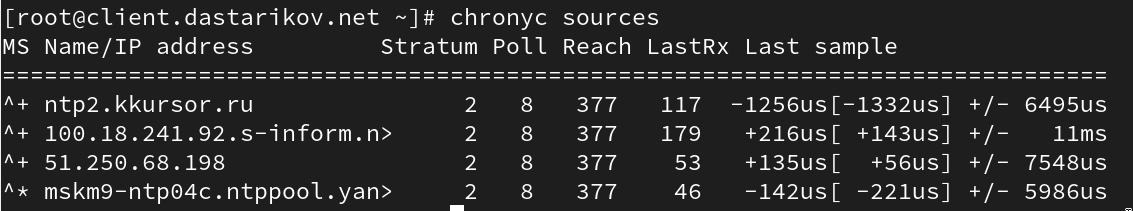
\includegraphics[width=\textwidth]{../images/image09.png}
    \captionof{figure}{Проверка источников времени на клиенте.}
\end{frame}

\begin{frame}[fragile]
\frametitle{Управление синхронизацией времени}
На сервере открыли на редактирование файл \texttt{/etc/chrony.conf} и добавили строку:
  \begin{minted}{bash}
    allow 192.168.0.0/16
  \end{minted}
    \centering
    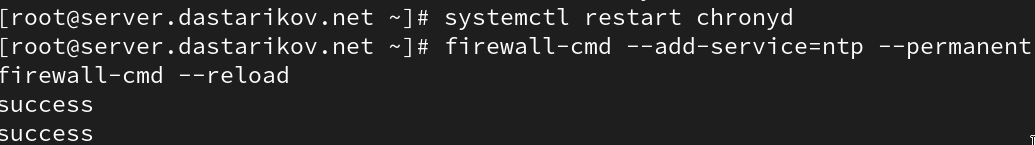
\includegraphics[width=\textwidth]{../images/image11.png}
    \captionof{figure}{Перезапуск \texttt{chronyd} и настройка межсетевого экрана.}
\end{frame}

\begin{frame}
\frametitle{Управление синхронизацией времени}
\centering
    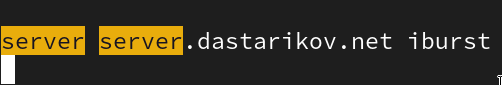
\includegraphics[width=\textwidth]{../images/image12.png}
    \captionof{figure}{Изменение файла конфигурации \texttt{chrony}.}
\end{frame}

\begin{frame}
\frametitle{Управление синхронизацией времени}
    \centering
    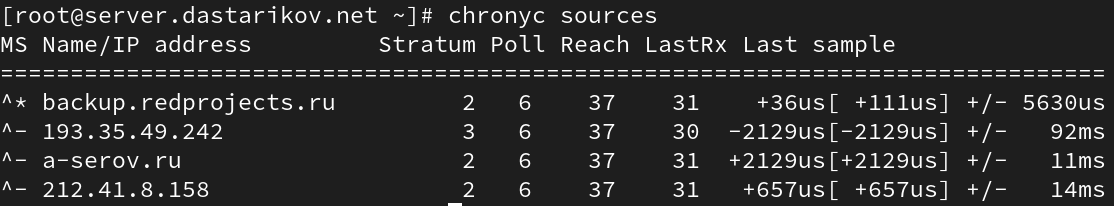
\includegraphics[width=\textwidth]{../images/image14.png}
    \captionof{figure}{Просмотр источников времени на сервере.}
\end{frame}

\begin{frame}
\frametitle{Управление синхронизацией времени}
    \centering
    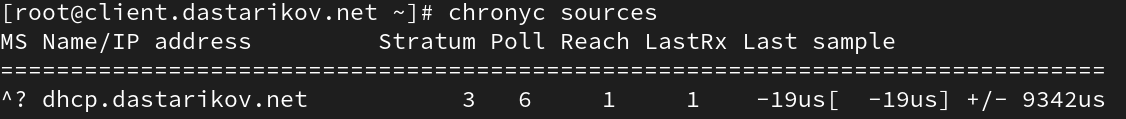
\includegraphics[width=\textwidth]{../images/image15.png}
    \captionof{figure}{Проверка добавленного источника времени на клиенте.}
\end{frame}

\begin{frame}
\frametitle{Внесение изменений в настройки внутреннего окружения виртуальных машин}
    \centering
    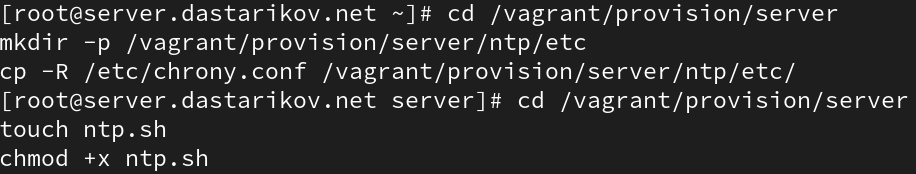
\includegraphics[width=\textwidth]{../images/image16.png}
    \captionof{figure}{Настройка внутреннего окружения виртуальной машины сервера.}
\end{frame}

\begin{frame}[fragile]
\frametitle{Внесение изменений в настройки внутреннего окружения виртуальных машин}
  \begin{minted}{bash}
    #!/bin/bash
    echo "Provisioning script $0"
    echo "Install needed packages"
    dnf -y install chrony
    echo "Copy configuration files"
    cp -R /vagrant/provision/server/ntp/etc/* /etc
    restorecon -vR /etc
    echo "Configure firewall"
    firewall-cmd --add-service=ntp
    firewall-cmd --add-service=ntp --permanent
    echo "Restart chronyd service"
    systemctl restart chronyd
  \end{minted}

\end{frame}

\begin{frame}
\frametitle{Внесение изменений в настройки внутреннего окружения виртуальных машин}
    \centering
    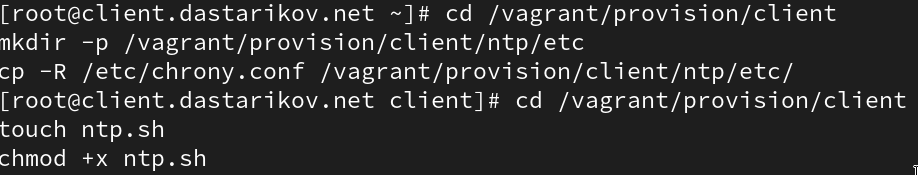
\includegraphics[width=\textwidth]{../images/image18.png}
    \captionof{figure}{Настройка внутреннего окружения виртуальной машины клиента.}
\end{frame}

\begin{frame}[fragile]
\frametitle{Внесение изменений в настройки внутреннего окружения виртуальных машин}
  \begin{minted}{bash}
    #!/bin/bash
    echo "Provisioning script $0"
    echo "Copy configuration files"
    cp -R /vagrant/provision/client/ntp/etc/* /etc
    restorecon -vR /etc
    echo "Restart chronyd service"
    systemctl restart chronyd
  \end{minted}
\end{frame}

\begin{frame}[fragile]
\frametitle{Внесение изменений в настройки внутреннего окружения виртуальных машин}
  \begin{minted}{bash}
    server.vm.provision "server ntp",
    type: "shell",
    preserve_order: true,
    path: "provision/server/ntp.sh"
    client.vm.provision "client ntp",
    type: "shell",
    preserve_order: true,
    path: "provision/client/ntp.sh"
  \end{minted}
\end{frame}

\begin{frame}
\frametitle{Выводы}
\begin{itemize}
    \item В результате выполнения лабораторной работы получили навыки по управлению системным временем и настройке синхронизации времени.
\end{itemize}
\end{frame}
\end{document}
